\section{Aufbau und Durchf"uhrung}
	\label{sec:durchfuehrung}

	Wir wollen die Halbwertszeiten $T$ f"ur ${}_{49}^{116}\mathrm{In}$ (Indium) und ${}_{45}^{104}\mathrm{Rh}$, bzw. ${}_{45}^{104i}\mathrm{Rh}$ (Rhodium) bestimmen.

	\subsection{Aufbau}
		\label{subsec:aufbau}
		F"ur diesen Versuch stand ein Geiger-M"uller-Z"ahlrohr (GMZ), sowie eine Z"ahluhr zur Verf"ugung.
		Die Proben wurden in das GMZ gegeben und die Uhr auf ein bestimmtes Zeitintervall $\Delta t$ eingestellt.
		Alle Zerf"alle, die das GMZ registrierte, wurden durch das Z"ahlwerk gez"ahlt.
		Die Anzeige wurde nach dem eingestellten Zeitintervall automatisch gel"oscht und die n"achste Z"ahlung begonnen.
		Um die Werte bequem ablesen zu k"onnen, besa"s die Z"ahluhr zwei Anzeigen, die abwechselnd eingeschaltet wurden.
		Folgende Ab\-bil\-dung zeigt den Aufbau:

		\begin{figure}[!h]
			\centering
			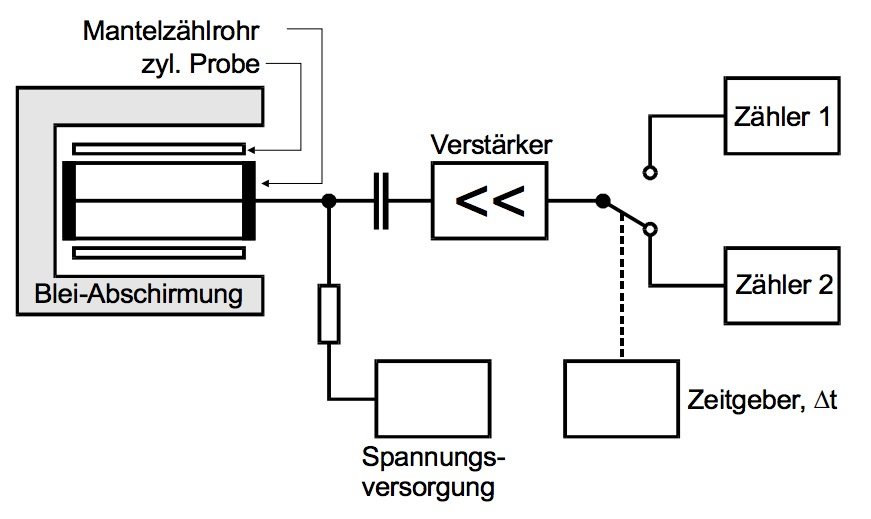
\includegraphics[width = 10cm]{img/aufbau.jpg}
			\caption{Versuchsaufbau \cite{anleitung}}
			\label{fig:aufbau}
		\end{figure}

	\subsection{Messaufgaben}
		\label{subsec:aufgaben}
		\begin{enumerate}
			\item{Bestimmung der Halbwertszeit $T_\mathrm{In}$ von Indium-116}
			\item{Bestimmung der Halbwertszeiten $T_{\mathrm{Rh}, 1}$ von Rhodium-104 und $T_{\mathrm{Rh}, 2}$ von Rhodium-104i}
		\end{enumerate}